% !TeX root = ../SPL-Challenges.tex
% !TeX spellcheck = en_US
\section{KICKin' \& Rollin' Challenge}

The objective of this challenge is for a robot to successfully kick a rolling ball from a ramp into a designated goal area. 
Each participating team will record three sessions, with a significant time between them.
A more specific schedule will be communicated closer to the competition.
A session consist of three kicks. 

\subsection{Field Setup}
\label{sec:field-setup}

\begin{figure}[t]
    \centerline{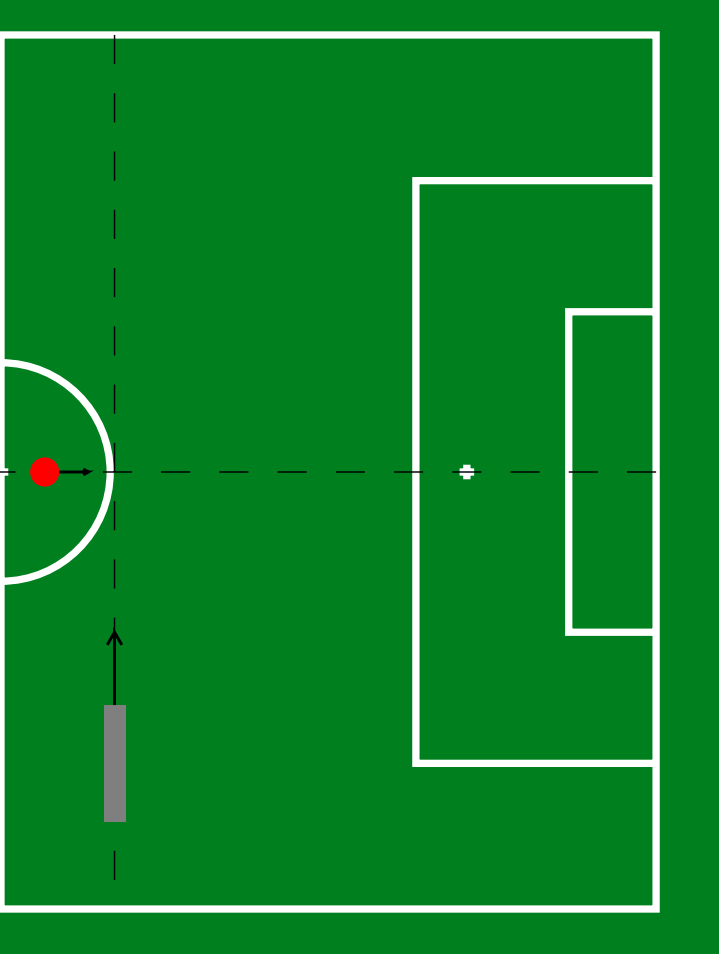
\includegraphics[width=\columnwidth/2]{figs/KICKin-Rollin-Placement-figure.png}}
    \caption{Illustration of robot and ramp placement for the challenge: The robot is depicted as a red dot, while the ramp is shown as a grey rectangle.}
    \label{fig:KICKin-Rolling-Challenge}
\end{figure}

The challenge will take place on a standard SPL field with its official marking. 
The ramp will be positioned on the virtual vertical line as show in \cref{fig:KICKin-Rolling-Challenge}.
The general idea is to position the Nao facing the goal, with the ball moving from its left to its right, or vice versa.
The ramp can be positioned at varying distances from the robots to modify the difficulty.
However, a minimum distance of 30 cm between the ramp and the virtual horizontal line (\cref{fig:KICKin-Rolling-Challenge}) must be maintained to ensure the ball rolls directly onto the field.
The participating robot can be positioned at the team’s discretion along the virtual horizontal line.
The robot must have one foot on each side of this virtual line.
The ball may not roll in a straight line due to field imperfections.
Teams need to adapt to the field conditions. 

\subsubsection{Ramp}

The selected ramp design will be made available on the SPL website. 
It may feature an adjustable angle to allow for modifications in difficulty.  

Teams are encouraged to propose their own ramp designs. 
For more information, visit the \url{https://spl.robocup.org/kickin-rollin-challenge-ramp/}.

\subsection{Challenge Procedure}

At the scheduled time, all participating teams must assemble on the designated field.
The ramp will be set up by the technical committee and will remain the same for all kicks executed this day.
Each team will perform their three kicks successively.
Teams are responsible for positioning their robots in accordance with \cref{sec:field-setup}.
The ready signal must be triggered manually using a sequence of sensors or buttons, at the team’s discretion.
This manual input may also be used to indicate the position of the ramp to the robot.
Network communication is strictly prohibited.
The robot is free to move after the manual input until the kick has been executed or the ball has stopped moving.
After the kick, whether successful or not, the team must pick up the robot and reset it for any remaining kicks in the session.
Teams may bring as many robots as needed, but they will not be allowed to deploy code between kicks.

\subsection{Scoring}

Each kick will receive a score based on the location of the ball.
These points are non-cumulative: 

\begin{itemize}
	\item 0 points for a missed kick or an undetected ball.
	\item 1 point for a deflected ball.
	A ball is considered deflected if it changes direction due to contact with the robot's feet.
	\item 2 points for kicking the ball.
	A ball is considered kicked if it makes contact with the front sensor of the robot's feet.
	\item 3 points for the ball entering the penalty area during the kick. 
	If the ball leaves the area before coming to a complete stop, without qualifying for subsequent points, this still counts. 
	\item 5 points for the ball entering the goal. 
	\item 100 points for the ball going over the goal between the virtual planes of the two goalposts. 
  \end{itemize}

  A ball can only be considered kicked or deflected if it result from a direct action by the robot.
  Contact resulting from a stationary feet or a backward step will result in 0 points.

  \subsection{Ranking}

  Each team will be ranked based on the average of their best kick from each session.